\documentclass[border=10pt]{standalone}

\usepackage{tikz}
\usepackage{tikzsymbols}
\usetikzlibrary{calc,patterns,shapes.geometric}

\def\centerarc[#1](#2)(#3:#4:#5){\draw[#1] ($(#2)+({#5*cos(#3)},{#5*sin(#3)})$) arc (#3:#4:#5);}

\begin{document}
	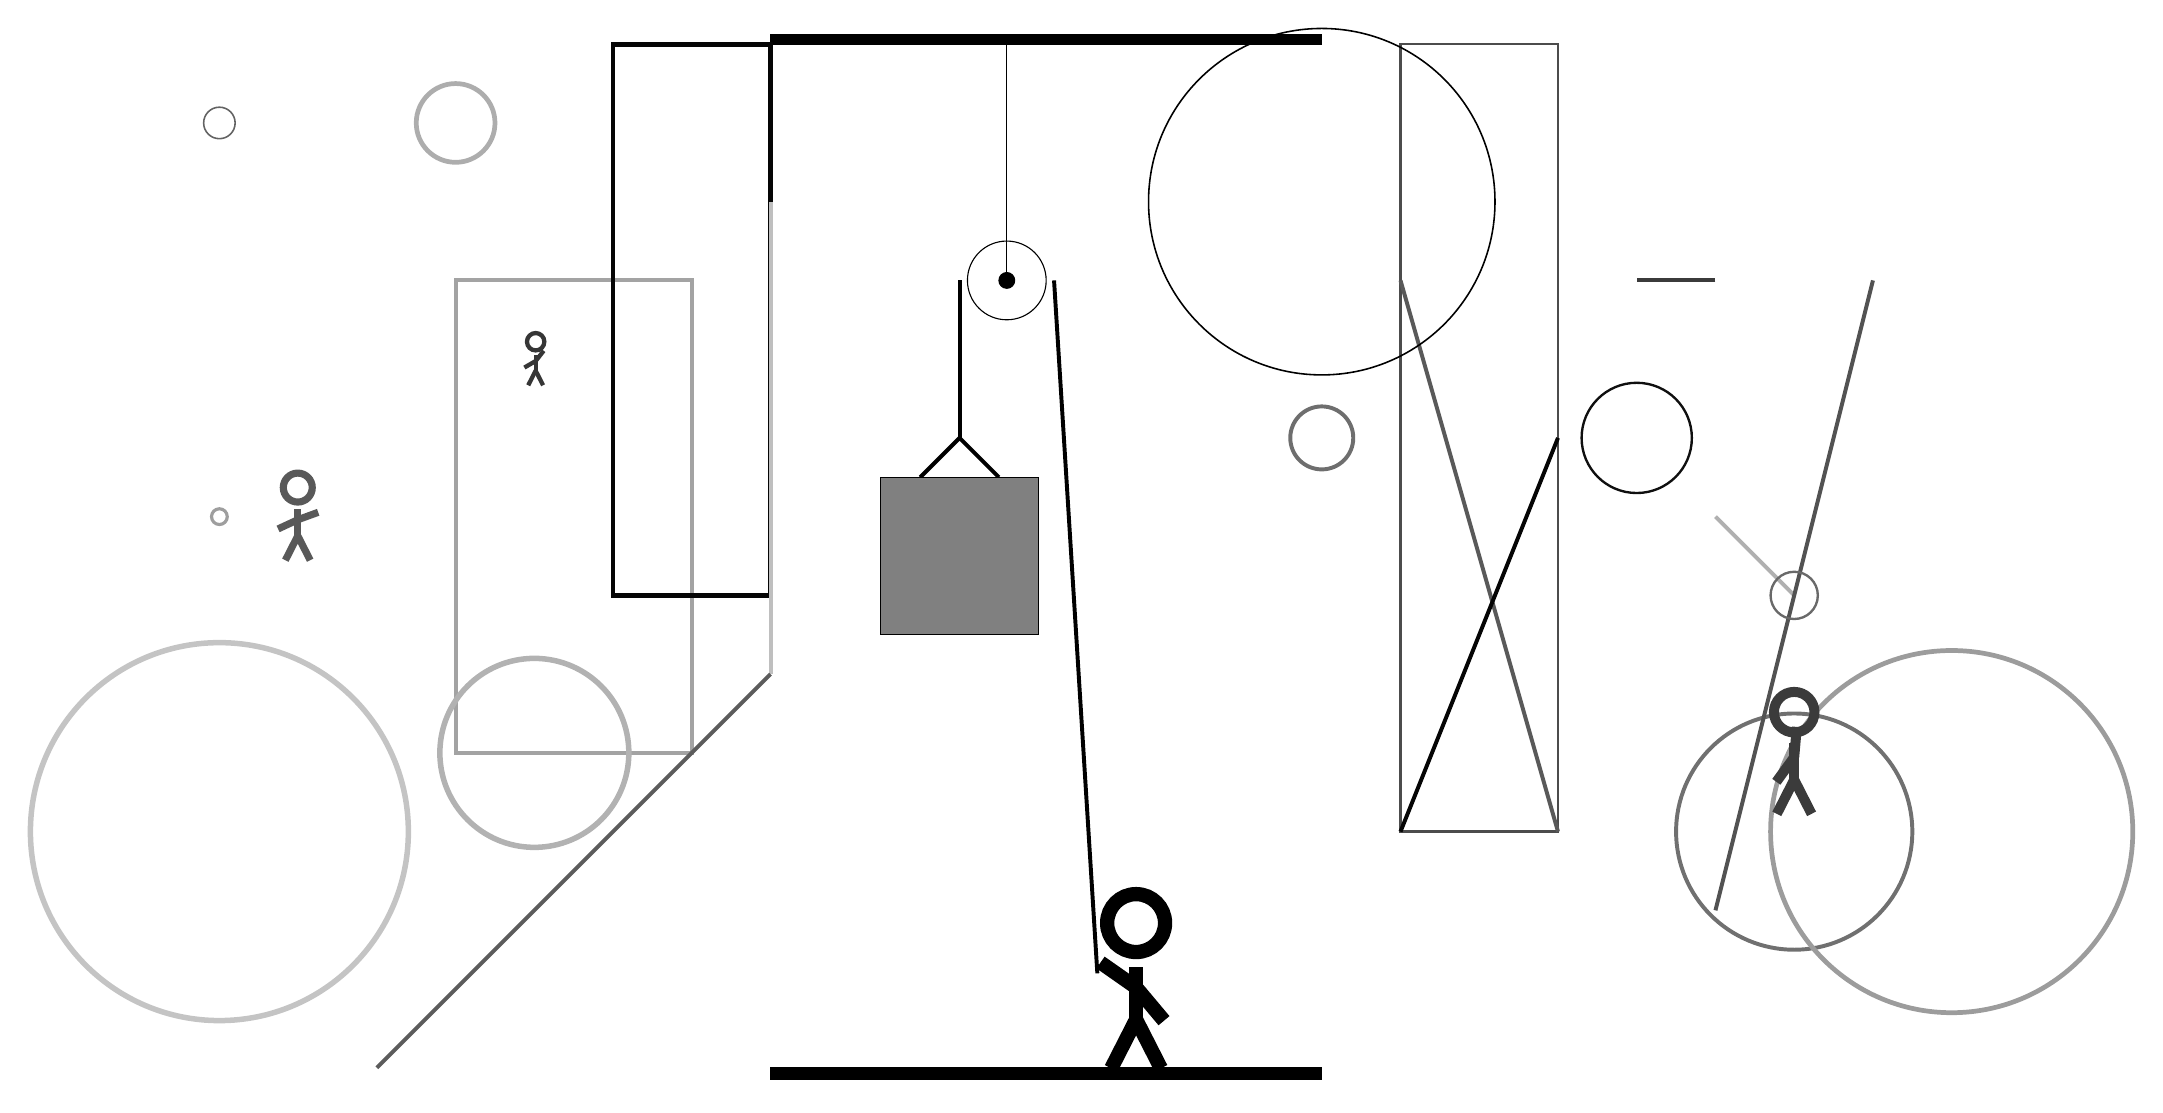
\begin{tikzpicture}
		%%%%% START %%%%%
		
		\draw[fill=black] (-2, 10) rectangle (5, 10.125);
		
		\draw (1, 7) circle (0.5);
		\draw[fill=black] (1, 7) circle (0.1);
		\draw (1, 10) -- (1, 7);
		
		\draw[line width=0.5mm] (-0.1, 4.5) -- (0.4, 5.0) -- (0.9, 4.5);
		\draw[fill=black!50] (-0.6, 4.5) rectangle (1.4, 2.5);
		
		\draw[line width=0.5mm] (0.4, 7) -- (0.4, 5.0);
		\centerarc[line width=0.5mm](1, 7)(0:180:0.6);
		\draw[line width=0.5mm](1.6, 7) -- (2.15, -1.8);
		
		\node at (2.6, -1.9) {\Strichmaxerl[10][-35][-50]};
		
		\draw[line width=0.5mm, color=black!36] (-3, 1) rectangle (-6, 7);
		
		\draw[line width=0.5mm, color=black!31](10, 4) -- (11, 3);
		\draw[line width=0.7mm, color=black!22] (7, -1) rectangle (7, -1);
		\draw [line width=0.5mm, color=black!56](11, 0) circle (1.5);
		\draw [line width=0.7mm, color=black!30](-5, 1) circle (1.2);
		
		\draw[line width=0.6mm, color=black!98] (-4, 3) rectangle (-2, 10);
		
		\draw [line width=0.7mm, color=black!23](-9, 0) circle (2.4);
		
		\draw[line width=0.5mm, color=black!25](-2, 2) -- (-2, 8);
		\draw[line width=0.5mm, color=black!64](-7, -3) -- (-2, 2);
		
		\draw [line width=0.6mm, color=black!39](13, 0) circle (2.3);
		\draw [line width=0.4mm, color=black!38](-9, 4) circle (0.1);
		\draw[line width=0.3mm, color=black!70] (6, 10) rectangle (8, 0);
		\draw[line width=0.5mm, color=black!65](6, 7) -- (8, 0);
		\draw[line width=0.5mm, color=black!68](10, -1) -- (12, 7);
		\draw [line width=0.2mm, color=black!61](-9, 9) circle (0.2);
		\draw[line width=0.5mm, color=black!77](10, 7) -- (9, 7);
		
		\draw[line width=0.5mm, color=black!98](6, 0) -- (8, 5);
		\node[line width=0.4mm, color=black!79] at (-5, 6) {\Strichmaxerl[3][30][52]};
		\draw [line width=0.3mm, color=black!59](11, 3) circle (0.3);
		\draw [line width=0.2mm, color=black!100](5, 8) circle (2.2);
		\draw [line width=0.5mm, color=black!57](5, 5) circle (0.4);
		\node[line width=0.7mm, color=black!77] at (11, 1) {\Strichmaxerl[7][54][85]};
		
		\draw [line width=0.3mm, color=black!94](9, 5) circle (0.7);
		\draw [line width=0.6mm, color=black!32](-6, 9) circle (0.5);
		\node[line width=0.3mm, color=black!65] at (-8, 4) {\Strichmaxerl[5][25][20]};
		
		
		\draw[fill=black] (-2, -3) rectangle (5, -3.15);
		
		%%%%% END %%%%%
	\end{tikzpicture}
\end{document}